\chapter{Metastability and phononic CDW quench in \ce{TaTe2}}

Collective phenomena arising from complex many body interactions have been a fascinating research topic for many decades.
One such example is the collective motion and ordering of electron-hole pairs, the so called charge density wave (CDW), which was first proposed in 1955 by Peierls \cite{peierls_quantum_1996} and has always been closely linked to the concept of superconductivity \cite{frohlich_theory_1997}.
This concept of CDWs found more traction when the first materials where found to host such exotic phases some decades after the first theoretical description.
The first experimental observations of CDWs were then found in pioneering works on blue bronzes by Fogle and Perlstein \cite{fogle_semiconductor--metal_1972} and in transition metal trichalocogenides by Monceau \cite{monceau_electric_1976}.

During the following decade many systems were found to exhibit CDW phases, and a high effort was focused on the understanding of CDWs, as is evident by the large amount of publications and reviews within that period \cite{wilson_questions_1978,gruner_dynamics_1988,yoffe_electronic_1990,wilson_charge-density_2001}.
In particular transition metal chalocogenides gathered attention, which arose from the many exotic properties next to CDWs found in the materials, as well as the fact that these were layered materials.
It was already shown in 1963 that ultrathin layers of the transition metal dichalcogenide (TMD) \ce{MoS2} could be exfoliated \cite{frindt_physical_1997}, and first monolayers were created in 1986 \cite{joensen_single-layer_1986}.
At the same time research on another layered material, graphite, resulted in the development of graphene monolayers.
This ultimately lead to stark research interest in layer engineering of e.g. nanotubes in graphene or \ce{WS2} and \ce{MoS2} \cite{iijima_helical_1991,tenne_polyhedral_1992,feldman_high-rate_1995}.

The problem of these materials lies in their strongly correlated many body nature, resulting in a very high complexity, making it difficult to predict and understand their properties.
The developments of the previous decades and especially the high interest in graphene-related topics lead to the introduction of graphene as a model system for more complex materials \cite{novoselov_electric_2004, novoselov_two-dimensional_2005, geim_rise_2007}.
Since then, researchers were extremely successful in finding new physical properties of graphene itself while also extending and applying the knowledge to other materials.
Apart from the simplicity of these 2D materials, the idea of engineering properties by stacking multiple layers with different stacking orders or at twist angles offered the possibility of a vast playground for discovering and engineering new properties.
This resulted in the explosion of the field with the discovery of many new phenomena, from the observation of quatum Hall effect \cite{zhang_experimental_2005} to superconductivty in magic angle twisted bilayer graphene \cite{cao_unconventional_2018}.

Ultimately these developments increased the desire for similar materials as an engineering and research platform.
One of these platforms of 2D materials are transition metal dichalcogenides (TMDs) \cite{butler_progress_2013, chowdhury_progress_2020, liu_van_2016}.
The development of such multilayer stacks of different TMDs, or the introduction of twist-angles resulted in a renaissance in the field of TMDs, as well as in the research of CDWs.
These layered TMDs are not only of interest because of the existence of CDWs, but rather a plethora of different exotic phases and phenomena like optoelectronic control, topological phases, superconductivity and the formation of excitons \cite{jiang_interlayer_2021, schmitt_formation_2022, mak_photonics_2016, koppens_photodetectors_2014, manzeli_2d_2017}.
Especially the coexistence and competition between charge density waves and superconductivity are a focal point in the understanding of high temperature superconductivity.

Since the 80s, the research on CDWs in TMDs was centered around the \ce{TaX2} based compounds \ce{TaS2} and \ce{TaSe2}.
Compared to these, the sister compound \ce{TaTe2} has received much less attention from the community, but multiple reports characterizing the compound have come up in recent years, especially due to it's strange behavior when crossing the CDW phase transition.
In this chapter of the thesis I will present static and trARPES data on \ce{TaTe2}, with the purpose of investigating the driving mechanism of the CDW formation and the structural phase transition.
First I will introduce the general concept of CDWs in 1D systems and the problems that arise at higher dimensions and strong couplings and will provide a small review on CDWs in the \ce{TaX2} compounds.
I will then introduce the band structure of \ce{TaTe2} and its Fermi surface topology, as well as comparing the high and low temperature phases, including the formation of CDW minigaps (first observed by \cite{lin_evidence_2022}).
After this I will give a description of the ultrafast charge dynamics on a few picosecond timescale, which includes the delayed melting response of the CDW.
The femtosecond light excitation is accompanied by strong, band specific oscillations.
These oscillations will be discussed in terms of their frequency, as well as energy and momentum resolved coupling between phonons and electrons.
Last, I present a metastable electronic state persisting for $>\qty{200}{\pico\second}$ and discuss it's relevancy for the structural phase transition at equilibrium.

\section{Charge Density Waves in strongly correlated matter}
\label{sec:cdw}


Charge density waves are collective modulations of the electron density, in which electron-hole pairs can form a condensate and behave like a macroscopic quantum state.
Additionally, CDWs are always accompanied by a periodic distortion of the lattice due to the coupling of electrons and phonons.
The concept of CDWs and PLDs has first been postulated by Peierls in 1955 \cite{peierls_quantum_1996} for the case of a 1D atomic chain.
Since then, a lot of effort was spent on understanding the mechanisms of CDWs on a microscopic level, and is now well understood for the 1D case.
The challenge arises when the dimensionality is increased and strong couplings come at play.
For those cases the understanding is much lower and is a topic of current research and intense debate.
In this section I will do short description of the 1D CDW as postulated by Peierls and after introduce the complications that arise from higher dimensionality and strong couplings, with a special focus on TMDs.
In recent years extensive reviews on the subject of CDW with a focus on TMDs have been published, which were used as a foundation this and the following section \cite{rossnagel_origin_2011, canadell_importance_1992}.

\begin{figure}[t]
	\centering
	\begin{subfigure}[b]{0.45\textwidth}
		\includegraphics[width=\textwidth]{tate2/lindhard.png}
	\end{subfigure}
	\hfill
	\begin{subfigure}[b]{0.5\textwidth}
		\includegraphics[width=\textwidth]{tate2/nesting_sketch.pdf}
	\end{subfigure}
	\\
	\begin{subfigure}[b]{0.9\textwidth}
		\includegraphics[width=\textwidth]{tate2/pld_cdw_sketch_mod.pdf}
	\end{subfigure}
	\caption{(a) 1T' RT phase of \ce{TaTe2} forming ribbons. (b) 1T" LT phase of \ce{TaTe2}, \ce{Ta} atoms move together forming heptameres. (c) Resistivity of \ce{TaTe2} as a function of temperature with an overall reduction in resistivity while cooling. A phase transition occurs at \qty{170}{\kelvin}, which is accompanied by a further steplike reduction in resistivity.}
	\label{fig:cdw_theory}
\end{figure}

Starting from the 1D atomic chain of a metal with a lattice spacing $a$, a cosinusoidally modulated electron density can be described by
\begin{equation}
	\rho(\mathbf{r}) = \rho_0(\mathbf{r})[1+\rho_1 \cos(\mathbf{q}_0\mathbf{r}+\phi)]
	\label{eq:cdw}
\end{equation}
with the unperturbed electron density $\rho_0$, $\rho_1$ the amplitude, $q_0$ the wavevector and $\phi$ the phase of the electron density modulation.
$\rho_1 \cos(\mathbf{q}_0\mathbf{r}+\phi)$ from above's equation represents the CDW and is a standing wave of wavelength $\lambda_0 = 2\pi/\lvert \mathbf{q}_0\rvert$.
The modulation of the charges as a function $\mathbf{r}$ results in an effective potential, with each ion feeling the presence of a different part of said potential.
This results in the ions moving away from their respective equilibrium position, in order to accommodate this new modulated potential.
The result of this movement is a distorted lattice, which is referred to as a periodic lattice distortion (PLD), which is of the form
\begin{equation}
	u_n = u_0 \sin(n\lvert \mathbf{q}_0\rvert a+\phi)
	\label{eq:pld}
\end{equation}
with the integer number $n$ describing the atom position and the amplitude of the distortion $u_0$.
Figure \ref{fig:cdw_theory} (c) shows a PLD of a 1D atom chain and the corresponding CDW.
While the mentioned case assumes an existing electron density modulation, or CDW, which then results in the formation of the PLD, the same equations will arise when starting from an existing PLD as in Eq. \ref{eq:pld}.
In that case, the existing PLD leads to a new effective potential, which the conduction electrons will try to screen, which will then result in a modulation of the charge density as described by Eq. \ref{eq:cdw}.
Therefore charge density waves and periodic lattice distortions always occur together \cite{rossnagel_origin_2011, chan_spin_1973, johannes_fermi_2008}.

The transition to a 1D CDW state as described by Peierls relies on the fact that the material is described as a Fermi liquid, with the electron gas only experiencing weak coupling with the ions via phonons.
In this picture the phonons connect different parts of the Fermi surface with momentum $+k_f$ and $-k_f$ (see Fig. \ref{fig:cdw_theory} (b)), which refers to Fermi surface nesting (FSN).
The connection of electrons with different Fermi momenta creates an instability at the Fermi surface, which drives a structural phase transition, mediated by the electron-phonon coupling.
Since the CDW formation and the FSN depend on the Fermi momenta ($k_f$), the CDW necessarily depends on the conduction band filling.
Additionally, the potential created by the CDW and PLD results in a gap opening at the Fermi level.
This potential is, for a given phonon mode $\mathbf{q}$ with the corresponding displacement $u_\mathbf{q}$, defined by
\begin{equation}
	v_\mathbf{q} = g_\mathbf{q} u_\mathbf{q} \sqrt{\frac{2M\omega_\mathbf{q}}{\hbar}}
\end{equation}
with the mass of the ion $M$.
Opening a gap at $E_F$ clearly lowers the energy of the occupied states while simultaneously increasing the energy of the unoccupied part of the band structure.
The energy change due to the gap opening caused by the potential $v_\mathbf{q}$ amounts to
\begin{equation}
	\delta E_{band} = -\lvert v_\mathbf{q}\rvert^2 \chi_0(\mathbf{q})
\end{equation}
with the non-interacting electronic susceptibility
\begin{equation}
	\chi_0(\mathbf{q}) = \frac{1}{L} \sum_{k}^{} \frac{f_{\mathbf{k}+\mathbf{q}}-f_\mathbf{k}}{\epsilon_\mathbf{k}-\epsilon_{\mathbf{k}+\mathbf{q}}}>0
	\label{eq:susz}
\end{equation}
$\chi_0$ represents therefore the net energy gain of the gapped band, and is dependent on the length of the atomic chain $L$ and the Fermi function $f(\epsilon_k)$ of the two nested states.
If the energy gain of the band exceeds the energy cost of the  strained lattice, which is given by
\begin{equation}
	\delta E_{lattice} = \frac{1}{2} M\omega_\mathbf{q}^2 u_\mathbf{q}^2
\end{equation}
than the CDW and PLD are self-sustaining and will be the new ground state of the system.

With the above equations in mind, and by including Coulomb and exchange interactions, it is possible to formulate a criterion \cite{chan_spin_1973}.
\begin{equation}
	\frac{4g_\mathbf{q}^2}{\hbar\omega_\mathbf{q}}-2U_\mathbf{q}+V_\mathbf{q}\geq\frac{1}{\chi_0(\mathbf{q})},
\end{equation}
for which a CDW state is formed.
This criterion indicates, that strong electron-phonon coupling $g_\mathbf{q}$, small Coulomb interaction, strong electron-electron interaction $V_\mathbf{q}$, small lattice strain energy $\omega_\mathbf{q}$ and a large $\chi_0(\mathbf{q})$ are the ingredients to form a CDW state.
The magnitude of aforementioned gap can be calculated by looking at the splitting of the normal-state band $\epsilon_\mathbf{k}$, assuming a tight-binding dispersion $\epsilon_\mathbf{k}=-E_F\cos(ka)$.
The splitting of the band occurs due to the fact, that the PLD superstructure wavevector $\mathbf{q}_0$ is equal to Fermi points $\pm\mathbf{k}_F$, which describe the Fermi nesting condition, which describes a energy discontinuity and the split band can be described by
\begin{equation}
	E_{1,2}(\mathbf{k})=\frac{\epsilon_{\mathbf{k}}+\epsilon_{\mathbf{k}+\mathbf{q}_0}}{2}\pm\sqrt{\left( \frac{\epsilon_{\mathbf{k}}+\epsilon_{\mathbf{k}+\mathbf{q}_0}}{2}\right)^2 + \Delta^2 }.
\end{equation}
$2\Delta$ represents the magnitude of the energy gap, which depends on the displacement amplitude of the PLD, the electron-phonon coupling $g_{\mathbf{q}_0}$ and the phonon frequency $\omega_{\mathbf{q}_0}$ \cite{gruner_density_2019}, with
\begin{equation}
	\Delta=u_{\mathbf{q}_0} + g_{\mathbf{q}_0} \sqrt{\frac{2M\omega_{\mathbf{q}_0}}{\hbar}}.
\end{equation}

Apart from the changes to the electronic band structure, the strong electron-phonon coupling also leads to a change of the phonon dispersion.
With a similar argument as before, the non-interacting susceptibility from Eq. \ref{eq:susz} diverges at low temperatures, when PLD wavevector $\mathbf{q}_0$ and nesting vector $2\mathbf{k}_F$ are equal.
$chi_0(\mathbf{q})$ can be expressed as a function of temperature and the density of states DOS$(E_F)$ at the Fermi level, which clearly indicates the diverging behavior
\begin{equation}
	\chi_0 (2\mathbf{k}_F, T)=\frac{1}{2}DOS(E_F)\ln\left( \frac{2.28E_F}{k_BT}\right).
\end{equation}
The divergence in the temperature dependent susceptibility indicates a renormalization of phonons in a wavevector in the range corresponding to $\mathbf{q}_0$, and is typically referred to as a Kohn anomaly.
The renormalized phonon can be expressed by
\begin{equation}
	\widetilde{\omega}_\mathbf{q}^2 = \omega_\mathbf{q}^2 \left( 1-\frac{4g_\mathbf{q}^2}{\hbar\omega_\mathbf{q}^2} \chi_0(\mathbf{q}) \right)
	\label{eq:kohn}
\end{equation}
and which reaches $0$ at finite temperatures $T_0$, if the electron-phonon coupling constant $g_{\mathbf{q}_0}>0$, resulting in the full softening of the phonon mode.

The finite temperature at which the phonon completely softens corresponds to the transition temperature between normal- and CDW-state.
From the equation \ref{eq:kohn} expressing the Kohn anomaly and by minimizing the total energy change of band and lattice $\delta E_{band}+\delta E_{lattice}$, it can be shown that, at $T=0$, the gap fulfills the following equation
\begin{equation}
	\Delta(0)=4E_F\exp(-\frac{1}{\lambda}),
\end{equation}
with the electron-phonon coupling constant $\lambda=\frac{2g_{\mathbf{q}_0}^2DOS(E_F)}{\hbar\omega_{\mathbf{q}_0}}$ \cite{rice_theory_1973}. 
Which leads to the famous Bardeen-Cooper-Schrieffer (BCS) relation, between the energy gap at zero temperature and the transition temperature
\begin{equation}
	2\Delta(0)=3.52k_BT_0.
\end{equation}

This description contains a full microscopic theory on CDW formation under the assumption of a 1D metal without the inclusion of electron-electron interactions.
Here it is important to mention, that for most materials these assumptions do not hold up.
The solution for the 1D chain, which predicts the long range order at a finite transition temperature $T_0$ does not hold for higher dimensions and is only relevant for quasi-1D systems.
Additionally, the Peierls instability at $E_F$ only materializes due to the exclusion of electron-electron interactions, expressed by the non-interacting susceptibility $\chi_0$.
With the interactions included, a material might be stable, even at the lowest temperatures.
Due to these facts, I will further discuss the consequences that higher dimensionality and strong electron-phonon coupling have on the CDW formation.
Both of which are the case for \ce{TaTe2}.

To recapitulate, in the 1D case the CDW formation is driven by the instability of the non-interacting susceptibility, which is a result of a coupling of many states with mode $\mathbf{q}$, most of which are coupled close to $E_F$.
While in 1D a metal has a planar Fermi surface, which can coincide for a given wavevector $\mathbf{q}$ with the $k_f$ points of the instability, this is not the case in 2D or 3D (see Fig. \ref{fig:cdw_theory} (b)).
Here the Fermi surface is generally not planar and the Brillouin zone edges do not intersect with the Fermi surface, which only results in a partial gap.
This partial gapping can occur when the Fermi surface of a 2D material behaves quasi-1D, where parts of the Fermi surface can be translated onto each other.
The result of the less ideal Fermi surface nesting in higher dimensions is that $\chi_0$ does not show a divergence at a specific wavevector $\mathbf{q}$ anymore, instead it rather shows a broader peak.
Figure \ref{fig:cdw_theory} (a) shows the Lindhard susceptibility from Eq. \ref{eq:susz} for a 1D, 2D and 3D case.
A broad peak in $\chi_0$ then requires stronger electron-phonon coupling to compensate for the smaller effect of $\chi_0$ in order to form a CDW.

Including stronger electron-phonon coupling, generally makes these observations even stronger.
A strong electron-phonon coupling generally leads to larger amplitude of the distortion and a larger energy gap, although the gap is larger its energy gain is not anymore concentrated to Fermi momenta $k_F$, but rather distributed across the whole Brillouin zone.
This shows further diminished factor that the Fermi surface nesting play in the formation of the CDW.
Another result of the stronger electron-phonon coupling lies in a shorter coherence length, which has implications for the way order is established in a CDW phase.
In the strong coupling regime order is established via local chemical bonds \cite{rossnagel_origin_2011, whangbo_analogies_1992, mcmillan_microscopic_1977,haas_chemical_1978,inglesfield_bonding_1980}.
Since the distortion amplitudes are larger, non-linear terms in the electron-phonon coupling become increasingly important, which results in the formation of pairs with shortened bonds or atom clusters.
The CDW will then tend to be commensurate with the distorted crystal lattice \cite{rossnagel_origin_2011}.
As will be further discussed in section \ref{sec:cdw_tate2}, the strong electron-phonon coupling will be an important factor for the description of the CDW phase in \ce{TaTe2}, which also tends to show strong local bonds.


\section{CDW phases in \ce{Ta}-based TMDs}
\label{sec:cdw_tate2}

As the previous section highlighted, higher dimensionality and stonger electron-phonon coupling complicates the situation and a microscopic description is lacking.
This situation is generally the case for TMDs, which typically show 2D behavior and exhibit stronger electron-phonon coupling.
From the \ce{Ta}-based TMDs, \ce{TaS2} and \ce{TaSe2} have experienced extensive research, while \ce{TaTe2} has only started to experience more attention in recent years.

Both \ce{TaS2} and \ce{TaSe2} show an undistorted monoclinic 1T phase at highest temperatures and undergo, multiple phase transitions \cite{pouget_structural_2024,lin_evidence_2022}.
\ce{TaS2} shows a transition from the normal state to a incommensurate CDW at around \qty{543}{\kelvin}, to a nearly commensurate CDW phase at \qty{352}{\kelvin}, to a finally commensurate CDW phase at \qty{183}{\kelvin}.
Similarly \ce{TaSe2} shows normal-state to incommensurate CDW transition only at \qty{122}{\kelvin} and a second transition to a commensurate CDW phase at \qty{90}{\kelvin}.
In the commensurate CDW phase of \ce{TaS2}, the \ce{Ta} atoms experience a strong modulation and form a cluster of 13 atoms in the shape of a "Star of David", while in \ce{TaSe2} only 7 atoms cluster together, which form the inner part of the "Star of David".

In contrast to these, \ce{TaTe2}-crystals form in orthorombic (1T) structures, although in bulk crystals the 1T-phase is only a virtual phase and only exists in a distorted 1T' phase up to highest temperatures measured ($>$\qty{500}{\kelvin}) \cite{petkov_exotic_2020}.
The 1T phase has only been realized in epitaxially grown mono and few-layer systems, which can form due to the absence of or only weakly existing \ce{Te}-\ce{Te} interlayer coupling \cite{hwang_novel_2022, wang_polymorphic_2024}.
In the real distorted 1T' phase, \ce{TaTe2} forms ribbon like structures and shows an overall (3 x 1) superstructure at the surface.
The structural distortion is governed by the local bonding, with \ce{Ta} atoms forming in trimers or fluctuating dimers, with each \ce{Ta}-atoms being surrounded by 8 \ce{Te}-atoms.
Additionally, the high temperature phase exhibits a commensurate stripe-like CDW phase.
At \qty{170}{\kelvin} the material undergoes a structural phase transitions, where two \ce{Ta}-atoms further distort the structure, breaking dimers and instead form "butterfly" shaped heptameres in a (3 x 3) 1T"-phase \cite{feng_charge_2016, katayama_observation_2023}.
Here, charge order is modulated and a hexagonal "star of david"-like charge order occurs below the phase transition, similar to \ce{TaSe2}.
This structural phase transition has been observed both in STM and diffraction measurements \cite{feng_charge_2016, siddiqui_ultrafast_2021, domrose_femtosecond_2024}.
Apart from the PLD, also the opening of gaps in the band tructure has been observed for all three compounds.
In \ce{TaSe2} a full gaps is opening at $E_F$, while for both \ce{TaS2} and \ce{TaTe2} the gap is not connected to the Fermi surface and is instead observed at higher binding energies \cite{lin_evidence_2022, mitsuishi_unveiling_2024}.

\begin{figure}
	\centering
	\begin{subfigure}[b]{0.3\textwidth}
		\includegraphics[width=\textwidth]{tate2/HT_tate_crystal.pdf}
	\end{subfigure}
	\hfill
	\begin{subfigure}[b]{0.3\textwidth}
		\includegraphics[width=\textwidth]{tate2/LT_tate_crystal.pdf}
	\end{subfigure}
	\hfill
	\begin{subfigure}[b]{0.3\textwidth}
		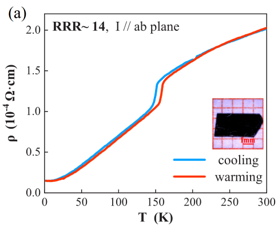
\includegraphics[width=\textwidth]{tate2/resistivity.png}
	\end{subfigure}
	\caption{(a) 1T' RT phase of \ce{TaTe2} forming ribbons. (b) 1T" LT phase of \ce{TaTe2}, \ce{Ta} atoms move together forming heptameres. (c) Resistivity of \ce{TaTe2} as a function of temperature with an overall reduction in resistivity while cooling. A phase transition occurs at \qty{170}{\kelvin}, which is accompanied by a further steplike reduction in resistivity. (a) and (b) adapted from \cite{lin_evidence_2022}, (c) from \cite{hu_optical_2022}.}
	\label{fig:tate_structure}
\end{figure}

As already mentioned before, \ce{TaS2} and \ce{TaSe2} are referred to as more prototypical CDW compounds, which show a Peierls-like instability, due to the fact that they show a PLD and opening of an electronic gap, as well as Kohn anomaly.
Even though all of these points are also true for \ce{TaTe2}, the phase transition in this compound is even more elusive.
The reason for the lack of understanding stems from the electronic reaction to the phase transition, especially in comparison to the \ce{TaX2} sister compounds.
Typically, as is the case for \ce{TaS2} and \ce{TaSe2}, entering a CDW phase by cooling the sample down from higher temperature leads to an increase in resistivity due to the reduced density of states (DOS) in proximity to the Fermi level $E_F$.
Similarly the loss in DOS and with it the loss of electrons carrying magnetic moments should lead to a drop of the magnetic susceptibility while cooling through $T_s$.
Instead \ce{TaTe2}, which inhibits semi-metallic behavior at RT, shows a drop in resistivity and an increase in magnetic susceptibility, despite the observation of small gaps in the band structure \cite{sorgel_new_2006,hu_optical_2022,lin_evidence_2022}.
For this reason the compound has been branded a "strange" CDW material.

The end of section \ref{sec:cdw} already discussed the problems that arise for higher dimensionality and stronger interactions.
While both \ce{TaS2} and \ce{TaSe2} are referred to as Peierls-like, the situation is more complicated than in the original 1D metal, postulated be Peierls.
Here the local-bonding picture becomes much more relevant and the role of the Fermi surface is reduced.
The local-bonding picture can be viewed as an analogy to molecular chemistry.
In TMDs for example, an electron deficiency leads to a charge transfer from the dichalcogenide to the transition metal, which leads to shortened bonds and clustering.
The charge transfer from \ce{Te} to \ce{Ta} allows for the formation of local multi-center bonds, forming the double zigzag patterns, which might be a driving force behind the PLD formation in \ce{TaTe2} \cite{pouget_structural_2024, whangbo_analogies_1992,canadell_importance_1992,albright_thomas_a_orbital_2013}.

In the next sections I will focus on the electronic band structure of \ce{TaTe2} and further discuss the formation of its CDW phase at LT with the help of trARPES data.
The local bonding picture, which has been mentioned in this section, will be important for the interpretation of the LT phase as well as the formation of a photo-induced metastable state.

\section{Bandstructure and Fermiology}

The electronic structure of \ce{TaTe2} is characterized by local molecular bonding of the Ta-Ta dimers, with ARPES measurements revealing a complex set of bands in the RT phase.
The valence states, which are governing the electronic properties of the compound consist of a mix of Ta 5d and Te 5p orbitals. \cite{mitsuishi_unveiling_2024}

The Fermi surface of \ce{TaTe2} shows a stronger quasi-1D character when compared to other 2D materials, even the isostructural \ce{TaSe2} and \ce{TaS2}.
This character can be observed by 2-fold symmetric wavy contours around \qty{0.5}{\angstrom^{-1}}, which are located along the $\Gamma$-M$_1$ direction and forms an outer Fermi surface.
Within these contours, an inner second Fermi surface forming multiple pockets can be located (see Fig. \ref{fig:TaTe_FS} (b)).

\begin{figure}[t!]
	\centering
	\begin{subfigure}[b]{0.49\textwidth}
		\includegraphics[width=\textwidth]{tate2/TaTe2_BZ_sketch_full.pdf}
		\caption{}
	\end{subfigure}
	\hfill
	\begin{subfigure}[b]{0.49\textwidth}
		\includegraphics[width=\textwidth]{tate2/TaTe2_contours.png}
		\caption{}
	\end{subfigure}
	\\
	\begin{subfigure}[b]{0.49\textwidth}
		\includegraphics[width=\textwidth]{tate2/TaTe2_FS_RT.pdf}
		\caption{}
	\end{subfigure}
	\hfill
	\begin{subfigure}[b]{0.49\textwidth}
		\includegraphics[width=\textwidth]{tate2/TaTe2_FS_LT.pdf}
		\caption{}
	\end{subfigure}
	\caption{(a) The measured Fermi surface of the LT phase is overlapped with the 1. BZ of the virtual monoclinic (1 x 1) 1T phase (black), extended BZs of the distorted HT (3 x 1) 1T' phase (orange) and extended BZs of the further distorted LT (3 x 3) 1 T'' phase (red). (b) LT Fermi surface shown together with the contours of the inner and outer Fermi surface sheet for which nesting conditions can be fulfilled (c) RT Fermi surface overlapped with the HT and LT Brillouin zones. The relevant high symmetry points are marked. (d) Same Fermi surface as (c) but measured in the LT phase at \qty{77}{\kelvin}.}
	\label{fig:TaTe_FS}
\end{figure}

Comparing the RT and LT Fermi surface, only small changes can be observed.
The overall topology, consisting of the wavy outer contours and an inner FS sheet with multiple pockets, is conserved.
A main difference lies in the slightly varied size of the pockets in the inner sheet, as well as some more pronounced features in the 2nd BZ of the LT FS.
The difference in size of the pockets stems from a slightly shifted chemical potential, when cooling through the phase transition, which has also been observed by N. Mitsuishi et. al. \cite{mitsuishi_unveiling_2024}.

Instead of the small changes in the Fermi surface topology, the effects of the phase transition become apparent when investigating the bandmaps.
Here, we compare a series of bandmaps taken parallel to the K$_2$-$\Gamma$-K$_2$ direction from the $\Gamma$-point to the edge of the 2nd BZ, for both room and low temperature.

\begin{figure}[t!]
	\centering
	\includegraphics[width=0.9\textwidth]{tate2/TaTe2_RT_cuts.pdf}
	\caption{Series of cuts parallel to K$_1$-$\Gamma$-K$_1$, from $\Gamma$ to the BZ border. The location of the cuts in respect to the BZ is indicated in the FS of Fig. \ref{fig:TaTe_FS}. All cuts have been taken at RT, using the Helium $\alpha1$ line of a Helium lamp.}
	\label{fig:TaTe_RT_cuts}
\end{figure}

The RT bandmaps show a manifold of bands, with multiple bands crossing the Fermi level in each cut.
These Fermi crossings clearly show the two different Fermi sheets, with the crossing at the edge of the cut determining the wavy contours of the outer quasi-1D Fermi surface sheet, and the crossing close to the center of the band structure forming the 2nd, inner Fermi sheet.
Cooling the compound through the phase transition results in a complex reordering of the bands.
The broader bands from the RT phase split in multiple individual ones, with additional backfolded bands appearing.
Looking at the FS crossing of the inner sheet, the aforementioned size difference of the Fermi pockets becomes clearer.
Comparing the cuts of the RT phase to the equivalent LT cuts, it is possible to identify a small shift in the chemical potential $\mu$, which has also been reported by \cite{mitsuishi_unveiling_2024}.
Another difference between the two phases is a band flattening close to $E_F$ at energies above \qty{-0.6}{\electronvolt}.

\begin{figure}[h]
	\centering
	\includegraphics[width=0.9\textwidth]{tate2/TaTe2_LT_cuts.pdf}
	\caption{Series of cuts parallel to K$_2$-$\Gamma$-K$_2$, from $\Gamma$ to the BZ border. The cuts are the equivalent band maps to the RT one in Fig. \ref{fig:TaTe_RT_cuts}. All cuts have been taken at LT $\simeq$\qty{77}{\kelvin}, using the Helium $\alpha1$ line of a Helium lamp.}
	\label{fig:TaTe_LT_cuts}
\end{figure}

This flattening of the bands might stem from the established charge order in the LT phase,  which typically results in the opening of gaps and backfolded bands from the PLD.
To further address the CDW and the gap formation we have to revisit the quasi-1D character of the FS.
A nesting of the FS occurs when different parts of the Fermi surface can be connected by a reciprocal lattice vector which can translate the different parts on top of each other, as has been discussed in section \ref{sec:cdw}.
This Fermi surface nesting (FSN) leads then to charge instabilities close to the FS and can play a dominant role in the formation of CDWs.
The wavy contours of the outer FS sheet (see Fig. \ref{fig:TaTe_FS}) can be translated onto each other and it is possible to talk about a Fermi surface nesting effect.
Determining the distance between two points that are connected by this vector results in a length of approximately \qty{0.92}{\angstrom^{-1}}, which is comparable to the \qty{0.85}{\angstrom^{-1}} found by Y. Lin et al. \cite{lin_evidence_2022}.
A possible second FSN vector can be found for the inner FS sheet.
These bands show a stronger 1D character and the vector has a length of \qty{0.24}{\angstrom^{-1}}.
Both of these FSN vector lengths do not correspond to the periodicity of the PLD, which was found to be $simeq\qty{0.67}{\angstrom^{-1}}$.

Section \ref{sec:cdw} and section \ref{sec:cdw_tate2} have already touched on the subject of higher dimensionality and stronger couplings.
The consequences of both become apparent here, where despite multiple possibly nested pockets no matching lattice superstructure is observed.
Even in materials with long quasi-1D Fermi surfaces the role of FSN is greatly diminished, which is obvious from the mismatch of the two vector amplitudes.
While FSN might be contributing in the formation of the CDW, it is not the sole, or leading contribution to the formation of the LT phase.

As a result of the CDW formation small gaps can be observed across the Brillouin zone, most prominently close to the $\Gamma$-point \cite{lin_evidence_2022}.
Figure \ref{fig:TaTe_minigaps} shows a cut close to $\Gamma$, with a dashed box around the area in which the minigap formation occurs.
A zoom of this region better showcases these small gaps at the edge of the band map at around \qty{0.4}{\angstrom^{-1}}.
This band also connects to the wavy contours, which fulfill the FSN condition, which highlights that an interplay between FSN and the gap formation might still be relevant.

\begin{figure}[h!]
	\centering
	\includegraphics[width=0.7\textwidth]{tate2/TaTe2_CDW_minigaps.pdf}
	\caption{Left: Band map parallel to the K$_2$-$\Gamma$-K$_2$ direction close to the $\Gamma$-point. The dashed rectangle marks the region of which a zoom is provided. Right: Zoom of dashed rectangle region. The band map shows a faint signature of the observed minigaps \cite{lin_evidence_2022}.}
	\label{fig:TaTe_minigaps}
\end{figure}

\section{Ultrafast charge dynamics and CDW quench}
\label{sec:tate_dynamics}

Investigating the evolution of the electronic band structure after pump excitation provides insight into the relaxation dynamics, not only of an isolated electronic states, but also the collective response of the material out of equilibrium.
This is especially beneficial when investigating complex materials, where multiple many-body effects can be at play, which also influence each other.
While static techniques will see the overall effects present in the material, time resolved techniques can help to establish an hierarchy between the various phenomena, which can help discriminating between the different contributions.
Here in particular, performing pump-probe experiments at RT and LN temperature allows us to reveal differences between the two different structural phases.
Through out this chapter the excitation is created by a \qty{1.55}{\electronvolt} ultrashort laser pulse.
Here, I will first analyze measurements that have been performed in the low temperature phase at \qty{77}{\kelvin} and then switch to RT data to point out the differences due to the phase transition.

The LT cuts, presented in this section, have been measured parallel to K$_2$-$\Gamma$-K$_2$ direction at three different points in the LT FBZ ($\Gamma$, M$_1$ and in proximity of $\Gamma$).
Focusing on the cut close to $\Gamma$ it is possible to make out a complex band dynamics, which strongly depends on the region in the band structure.
Figure \ref{fig:TaTe_bandmap_dyn_betw} shows this band map \qty{50}{\femto\second} after excitation.
Additionally, difference maps for three different time steps (\qtylist{50; 500; 4000}{\femto\second}) are plotted to better visualize the pump-induced changes.

At \qty{50}{\femto\second} a fast depopulation of occupied bands can be observed, with the difference band contours following the band structure at equilibrium.
Similarly a fast population of the unoccupied states occurs.
It is important that the contours in the difference map follow the bands in the raw data, because it highlight the fact, that the intensity changes actually correspond to a change in population and not a relative band shift.
These dynamics are followed by an initial decay of the excitation, but at \qty{500}{\femto\second} a sudden increase in spectral weight occurs in the occupied states.
This atypical behavior can be explained by a quench of the charge order, and will be discussed in greater detail when analyzing specific delay traces at the end of this section.
But it is crucial to highlight that the region in which the raised intensity is observed, corresponds to the the region where CDW minigaps form.
At a time delay of \qty{4}{\pico\second} most of the population in the excited states has decayed, but a rest population is still observed.
Additionally the band structure is significantly altered compared to the equilibrium state.

\begin{figure}[t!]
	\centering
	\includegraphics[width=\textwidth]{tate2/bandmap_dyn_markers_betw.png}
	\caption{Left: Band map close to $\Gamma$ oriented along K$_2$-$\Gamma$-K$_2$ direction at a time delay of \qty{50}{\femto\second} after pump excitation. The other plots show difference maps at different time delays (\qtylist{50;500;4000}{\femto\second}). Rectangles show the regions for which dedicated delay traces are displayed in \ref{fig:TaTe_dyn_betw}. The difference map show characteristic features for each time steps. At \qty{50}{\femto\second} fast de-/population due to the pump excitation occurs. After \qty{500}{\femto\second} a population of a region below $E_F$ appears, corresponding to the closure of the CDW gap. After \qty{4}{\pico\second} the difference map shows regions where a change of the band structure and population above $E_F$ persists. Measurement was done at \qty{77}{\kelvin}.}
	\label{fig:TaTe_bandmap_dyn_betw}
\end{figure}

Some exemplary traces have been selected for a more detailed insight into the relaxation dynamics.
These traces are marked with squares in the band maps, black squares for the unoccupied band structure, white for the occupied region and green for the region with a significant spectral weight after \qty{4}{\pico\second}.
Traces for the unoccupied region (black squares, see Fig. \ref{fig:TaTe_dyn_betw} (a)-(c)) shows a sharp population within the duration of the pump pulse.
The ultrafast population is followed by a fast decay which becomes increasingly longer when approaching $E_F$.
In each trace, the population has decayed within \qty{4}{\pico\second}.
Similarly the depopulation of the occupied state in Fig. \ref{fig:TaTe_dyn_betw} (d) is created within the pump pulse duration and recovers on the same time scale.

Unexpected dynamics occur when looking at the region that shows an increase in population below $E_F$.
Typically a pump light pulse excites the system which transfers energy to electrons and drives a transition to a higher unoccupied state, therefore reducing the occupancy below $E_F$.
Instead \ce{TaTe2} shows small gaps resulting from the CDW, which leads to a loss of density of states (DOS) at equilibrium, when compared to the normal state.
If this charge order is broken, the gap closes and in a simple case, excluding other band modifications, the DOS of the RT phase is re-established.
This behavior is observed in Fig. \ref{fig:TaTe_dyn_betw} (e), which coincides with the region of CDW gaps reported by \cite{lin_evidence_2022}.
Strikingly, the breaking of the CDW order does not occur at $t_0$.
Fitting a single exponential decay model retrieves a time zero of $t_0=\qty{388}{\femto\second}$, introducing a significant delay of approximately \qty{320}{\femto\second} when compared to the time zero of all other curves.

\begin{figure}[t]
	\centering
	\begin{subfigure}[b]{0.33\textwidth}
		\includegraphics[width=\textwidth]{tate2/Unocc_dyn_1_fit_betw.pdf}
		\caption{}
	\end{subfigure}
	\hfill
	\begin{subfigure}[b]{0.33\textwidth}
		\includegraphics[width=\textwidth]{tate2/Unocc_dyn_2_fit_betw.pdf}
		\caption{}
	\end{subfigure}
	\hfill
	\begin{subfigure}[b]{0.33\textwidth}
		\includegraphics[width=\textwidth]{tate2/Unocc_dyn_3_fit_betw.pdf}
		\caption{}
	\end{subfigure}
	\\
	\begin{subfigure}[b]{0.33\textwidth}
		\includegraphics[width=\textwidth]{tate2/Occ_dyn_fit_betw.pdf}
		\caption{}
	\end{subfigure}
	\hfill
	\begin{subfigure}[b]{0.33\textwidth}
		\includegraphics[width=\textwidth]{tate2/CDW_quench_fit_betw.pdf}
		\caption{}
	\end{subfigure}
	\hfill
	\begin{subfigure}[b]{0.33\textwidth}
		\includegraphics[width=\textwidth]{tate2/Meta_dyn_fit_betw.pdf}
		\caption{}
	\end{subfigure}
	\caption{Delay traces of the regions marked in Fig. \ref{fig:TaTe_bandmap_dyn_betw} with the corresponding fit function of a single exponential decay model and resulting time constants $t_0$ and $\tau$. (a)-(c) Dynamics of unoccupied regions (black markers in Fig. \ref{fig:TaTe_bandmap_dyn_betw}) show fast population within pump pulse, followed with increasing relaxation time closer to $E_F$. (d)-(e) Dynamics of unoccupied regions (white markers in Fig. \ref{fig:TaTe_bandmap_dyn_betw}). (d) Fast depopulation within pump excitation. (e) Delayed response compared to $t_0$ and increased spectral weight. (f) Dynamics of region slightly above $E_F$ (green marker in Fig. \ref{fig:TaTe_bandmap_dyn_betw}) shows a instantaneous population within pump pulse, and persisting occupation beyond \qty{4}{\pico\second}.}
	\label{fig:TaTe_dyn_betw}
\end{figure}

This delayed response becomes very apparent, when the delay trace is overlapped with the dynamics of the fast population and depopulation (see Fig. \ref{fig:TaTe_CDW_comp}).
Many ultrafast studies have looked at the dynamics of the CDW and while the timescales typically differ, depending on the mechanism, a common observation is that the quench of the charge order starts together with the arrival of the pump pulse \cite{perfetti_time_2006, rohwer_collapse_2011, rettig_coherent_2014, shi_ultrafast_2019, maklar_nonequilibrium_2021, maklar_coherent_2022, huber_mapping_2022, huber_revealing_2022, maklar_coherent_2023, huber_ultrafast_2024}.
In contrast, here a quench on the timescale of few hundred \unit{\femto\second} is observed, which is typically associated with a Peierls type CDW, but the onset of the quench is delayed with respect to time zero $t_0$.
The delayed response rules out a solely electronic character and instead established the structural component as the dominant contribution for the CDW order in \ce{TaTe2}.
In other words, instead of the electromagnetic field of the pump pulse directly disrupting the charge order e.g. via buildup of free charges and subsequent screening, the more likely scenario is a coherent response of the lattice to the intense light illumination, resulting in an excitation of phonon modes on ultrafast time scales, which couple to the charge order via the strong electron-phonon coupling of the system.

The unresponsiveness of the CDW to the direct light illumination shows as well when looking at a region at the edge of the CDW gap, also containing the part of the gapped band.
The corresponding dynamics, overlapped with the dynamics of the direct de-/population are shown in Fig. \ref{fig:TaTe_CDW_comp}.
In the trace an inital dip at $t_0$ can be seen, originating from the depopulation dynamics of the occupied band.
But after \qty{300}{\femto\second}, this depopulation is drowned out by the closing of the CDW gap.
It is quite remarkable that in adjacent energy-momentum coordinates an instantaneous reaction to the occupied band dynamics is observed while the CDW only shows a delayed response, which speaks for the strong structural character of the established order.
A relaxation time of $\tau_{CDW}=\qty{500}{\femto\second}$ can be extracted by fitting a single exponential decay model, corresponding to the time duration to reestablish the charge order.

\begin{figure}[t!]
	\centering
	\begin{subfigure}[b]{0.33\textwidth}
		\includegraphics[width=\textwidth]{tate2/CDW_quench_multitrace_betw.pdf}
		\caption{}
	\end{subfigure}
	\begin{subfigure}[b]{0.33\textwidth}
		\includegraphics[width=\textwidth]{tate2/CDW_2_dyn_fit.pdf}
		\caption{}
	\end{subfigure}
	\caption{Left: Delay trace showing the dynamics of the CDW quench, overlapped with delay traces showing the direct de-/population of the occupied/unoccupied states, visualizing the delayed response of the CDW to the light excitation. Right: Dynamics of CDW quench combined with a fit of a single exponential decay model, resulting in a decay time of $\tau_{CDW}=\qty{460}{\femto\second}$ and an onset of the dynamic at $t=\qty{420}{\femto\second}$.}
	\label{fig:TaTe_CDW_comp}
\end{figure}

Coming back to the residual spectral weight visible in the difference map at \qty{4}{\pico\second} in Fig. \ref{fig:TaTe_bandmap_dyn_betw}, the corresponding delay trace of the green square (see Fig. \ref{fig:TaTe_dyn_betw}) shows the same fast population within the pump pulse duration, with an initial decay, but the population does not return to the initial state.
Instead a sharp feature is visible above $E_F$.
A more detailed analysis of this feature, including measurements on longer time scales, will be done in section \ref{sec:meta}.
Also a common feature in the delay traces are strong coherent oscillation of the intensity.
A detailed analysis of these oscillations will also be tackled in the next sectionm\ref{sec:phonon_osc}.

\begin{figure}[t!]
	\centering
	\begin{subfigure}[b]{\textwidth}
		\includegraphics[width=\textwidth]{tate2/bandmap_dyn_markers_gamma.png}
		\caption{}
	\end{subfigure}
	\\
	\centering
	\begin{subfigure}[b]{\textwidth}
		\includegraphics[width=\textwidth]{tate2/bandmap_dyn_markers_bzb.png}
		\caption{}
	\end{subfigure}
	\\
	\begin{subfigure}[b]{0.33\textwidth}
		\includegraphics[width=\textwidth]{tate2/CDW_quench_multitrace_gamma.pdf}
		\caption{}
	\end{subfigure}
	\begin{subfigure}[b]{0.33\textwidth}
		\includegraphics[width=\textwidth]{tate2/CDW_quench_multitrace_bzb.pdf}
		\caption{}
	\end{subfigure}
	\caption{Figure similar to Fig. \ref{fig:TaTe_bandmap_dyn_betw} for different cuts. (a) Cut through $\Gamma$. (b) Cut through M$_1$. Both cuts are along the K$_2$-$\Gamma$-K$_2$ direction. (c) \& (d) show trace of the CDW quench plotted together with the direct excitation of the unoccupied states.}
	\label{fig:TaTe_bandmap_dyn_bzb}
\end{figure}

This series of dynamics is not only visible in proximity to $\Gamma$ but can also be observed directly at $\Gamma$, as well as at the edge of the FBZ at M$_1$.
Figure \ref{fig:TaTe_bandmap_dyn_bzb} shows the excited bandmap at $t_0$, followed by difference maps at specific time delays.
In both, the same instantaneous de-/population of the occupied/unoccupied bands is visible, as well as a quench of a CDW gap that also shows a delayed response of multiple hundreds of \unit{\femto\second} (see Fig. \ref{fig:TaTe_bandmap_dyn_bzb} (c)-(d)).
The only difference in the dynamics is an absence of residual spectral weight at M$_1$, but this measurement has been performed at a lower pump fluence, which is the reason for the absence.

Comparing the dynamics of the LT phase to the RT phase, reveals significant differences for the same cut of band structure (see Fig. \ref{fig:TaTe_bandmap_dyn_betw_rt} cut close to $\Gamma$).
First a direct population of the occupied states can be observed within the pump pulse duration.
But, unlike the LT case, the population seems to be disproportionately located in the region just above $E_F$, whereas the unoccupied states at higher energies appear to be less populated.
While the LT phase was additionally characterized by strong changes to the band structure after the first few hundred \unit{\femto\second}, no changes occur in the RT phase.
Instead, the population of the unoccupied bands, as well as the depopulation of the occupied parts simply decays.
After \qty{3}{\pico\second} some spectral weight still remains close to $E_F$, but no discrete spectral feature can be observed.
The full time dynamic for selected regions, which are marked by squares in Fig. \ref{fig:TaTe_bandmap_dyn_betw_rt}, can be seen in Fig. \ref{fig:TaTe_dyn_betw_rt}.
Those traces show similar relaxation times as the LT ones.

\begin{figure}[t!]
	\centering
	\includegraphics[width=\textwidth]{tate2/diffmap_dyn_markers_betw_rt.png}
	\caption{Left: Band map close to $\Gamma$ oriented along K$_2$-$\Gamma$-K$_2$ direction \qty{50}{\femto\second} after pulse excitation. The other plots show difference maps at different time delays (\qtylist{50;400;3000}{\femto\second}). Rectangles show the regions for which dedicated delay traces are displayed in \ref{fig:TaTe_dyn_betw_RT}. The difference map shows the ultrafast de-/population after pump excitation, followed by a decay and a small diffuse residual spectral weight after \qty{3}{\pico\second}. No changes to the band structure apart from de-/population dynamics can be observed.}
	\label{fig:TaTe_bandmap_dyn_betw_rt}
\end{figure}

\begin{figure}[b!]
	\centering
	\begin{subfigure}[b]{0.24\textwidth}
		\includegraphics[width=\textwidth]{tate2/Unocc_dyn_1_fit_betw_rt.pdf}
		\caption{}
	\end{subfigure}
	\begin{subfigure}[b]{0.24\textwidth}
		\includegraphics[width=\textwidth]{tate2/Unocc_dyn_2_fit_betw_rt.pdf}
		\caption{}
	\end{subfigure}
	\begin{subfigure}[b]{0.24\textwidth}
		\includegraphics[width=\textwidth]{tate2/Unocc_dyn_3_fit_betw_rt.pdf}
		\caption{}
	\end{subfigure}
	\begin{subfigure}[b]{0.24\textwidth}
		\includegraphics[width=\textwidth]{tate2/Occ_dyn_fit_betw_rt.pdf}
		\caption{}
	\end{subfigure}
	\caption{
		Delay traces of the regions marked in Fig. \ref{fig:TaTe_bandmap_dyn_betw_rt} with the corresponding fit function of a single exponential decay model and resulting time constants $t_0$ and $\tau$. (a)-(c) Dynamics of unoccupied regions (black markers in Fig. \ref{fig:TaTe_bandmap_dyn_betw_rt}) show fast population within pump pulse, followed with increasing relaxation time closer to $E_F$. (d) Dynamic of unoccupied regions (white markers in Fig. \ref{fig:TaTe_bandmap_dyn_betw_rt}) shows fast depopulation within pump excitation and small residual spectral weight after \qty{3}{\pico\second}.}
	\label{fig:TaTe_dyn_betw_rt}
\end{figure}

With these results in mind, two key differences are apparent from the RT data.
First is the lack of a spectral feature appearing around \qty{500}{\femto\second}, as well as no band reordering.
Second, while there is still some residual spectral weight left after \qty{3}{\pico\second}, there are no sharp features visible.
Instead the spectral weight seems to have a diffuse distribution around the occupied bands.
Additionally, there is no band reordering associated with this residual spectral weight.

The differences show that HT phase is very resistant to photo-illumination, which has also been observed and discussed in the context of ultrafast structural studies \cite{domrose_femtosecond_2024}.
This absence of distinct spectral changes at HT is also remarkable, due to the fact that stripe-like charge ordering exists in the HT phase.
In contrast, the LT phase shows that the charge order can be melted with ultrafast light pulses, which can be seen from the increased population below $E_F$.
Additionally, ultrafast structural studies \cite{domrose_femtosecond_2024, siddiqui_ultrafast_2021} have reported on a partial melting of the PLD.
The complex reformation of bands might be as well a direct consequence of this.
The delayed response of the CDW quench speaks in favor of a strong structural character of the CDW/PLD.
Lastly,an observed residual spectral weight above $E_F$ is only observed in the LT phase, which indicates the existence of a metastable state.

As has been shown through out this section, the time dynamics change significantly with position in energy and momentum space.
The next section will discuss the momentum and energy dependent dynamics in greater detail.
Furthermore, the residual spectral weight will be discussed in terms of a metastable state in section \ref{sec:meta}.

\section{Energy and momentum resolved electron-phonon coupling}
\label{sec:phonon_osc}

The previous section was dedicated to the dynamics both at LT and RT.
Those dynamics already revealed strong momentum and energy dependent oscillations in the intensity of each trace, which will be the subject of this section.

Coherent oscillations in delay traces of a trARPES measurement typically are a sign of interaction with phonons.
Since ARPES only measures the single particle wavefunction of photoemitted electrons, it is not possible to directly observe quasiparticles like phonons.
Instead the information of phonons is imprinted onto the measured photoelectrons due to the electron-phonon coupling.
If this coupling becomes sufficiently large it is possible to observe oscillations in time traces of a trARPES experiment.
Multiple pathways to coherently excite phonons exist, with various Raman scattering processes, infrared absorption and displacive excitation of coherent phonon (DECP) being among them \cite{zeiger_theory_1992, kuznetsov_theory_1994, giret_entropy_2011,juraschek_sum-frequency_2018,lakehal_microscopic_2019,caruso_quantum_2023, emeis_coherent_2024}.
For semi-metals DECP is typically the main excitation pathway.
In this process, photons of the pump pulse are absorbed and the created photoexcitation results in a quasi-adiabatic displacement of the potential energy surface.
The lattice then reacts by oscillating around the minimum of the displaced energy surface in a coherent motion, which is slowly dephases over time dampening the phonon \cite{zeiger_theory_1992, kuznetsov_theory_1994, bothschafter_ultrafast_2013, emeis_coherent_2024}.

Ditellurides, and especially \ce{TaTe2} seem to carry an exceptionally high electron-phonon coupling.
Due to this, it is not only possible to observe oscillations in a large, integrated region of the band structure, but rather for each momentum and energy coordinate individually, which enables the possibility of performing band mappings of the electron-phonon coupling constant in a large energy-momentum region.
Additionally, by carrying out a Fourier analysis of the delay trace we can extract the frequency of the oscillation and assign it to known vibrational modes.
To the best of my knowledge, this is the first time such a Fourier analysis of the $E$ and $k$ resolved electron-phonon coupling has been done in ARPES using high harmonic generation as a probe.

\begin{figure}[b!]
	\centering
	\includegraphics[width=\textwidth]{tate2/tate_fit_procedure.pdf}
	\caption{Left: Band map close to $\Gamma$ oriented along K$_2$-$\Gamma$-K$_2$ direction \qty{50}{\femto\second} after pulse excitation. The other plots show difference maps at different time delays (\qtylist{50;400;3000}{\femto\second}). Rectangles show the regions for which dedicated delay traces are displayed in \ref{fig:TaTe_dyn_betw_RT}. The difference map shows the ultrafast de-/population after pump excitation, followed by a decay and a small diffuse residual spectral weight after \qty{3}{\pico\second}. No changes to the band structure apart from de-/population dynamics can be observed.}
	\label{fig:TaTe_fit_procedure}
\end{figure}

For this procedure a small binning of four pixel in both the momentum and energy coordinate is applied to the raw data to slightly increase the signal to noise ration and reduce the amount of pixels for which the calculations have to run, and only slightly sacrificing the fidelity of the bandmaps.
An analytic function reproducing the fast population or depopulation after pump excitation and subsequent decay of the excitation is fit to each $E(k)$-coordinate.
The analytic function is defined by
\begin{equation}
	A + \frac{1}{2} \left( B * \exp\left(\frac{t_0-t}{\tau} + \frac{\sigma}{\tau}\right) \right) * \left( 1 + \text{erf}\left(\frac{t-t_0-\frac{2\sigma}{\tau}}{\sigma*\sqrt{2}}\right) \right) + C \frac{1}{2} * \left( 1 + \text{erf}\left(\frac{t-t_0}{\sigma*\sqrt{2}}\right) \right)
	\label{eq:decay_model}
\end{equation}
with time zero $t_0$, decay time $\tau$ and a broadening $\sigma$.
erf represent the error function as defined by
\begin{equation}
	\text{erf}(z) = \frac{2}{\sqrt{\pi}} * \int_{t=0}^{z} \exp(-t^2)
\end{equation}
The exponential decay is then subtracted from the raw data trace, only leaving a residual behind containing the oscillating components.
A fast Fourier transform function from the scipy Python package \cite{noauthor_rfft_nodate} is then applied to the residual trace, revealing the frequency of the oscillatory components.
In the specific case here the datasets consist of 60 delay steps.
The FFT function was defined to consist of 200 points, therefore applying a zero padding of 140 points.
Applying the FFT function transforms the original 3D data cube from $I(E,k,t)$ to $I(E,k,f)$, with frequency $f$ being the Fourier transformed of the time axis.
Fig. \ref{fig:TaTe_fit_procedure} shows the steps from a delay trace to the FFT trace that can be associated with a particular phonon mode.

Performing this analysis for a cut close to $\Gamma$ reveals 3 distinct vibrational modes in the LT phase (see Fig. \ref{fig:TaTe_FFT_betw} (c)) at \qtylist{0.4; 1.45; 2.3}{\tera\hertz}.
Two modes (\qtylist{1.45; 2.3}{\tera\hertz}) are well known phonon modes which have been observed with Raman spectroscopy and ultrafast transient reflectivity \cite{luo_subtle_2021, hu_optical_2022}, while the \qty{0.4}{\tera\hertz} on the other hand has not been observed.
The resulting band maps for these three frequencies are shown in Fig. \ref{fig:TaTe_FFT_betw} (b) with the corresponding band structure \qty{50}{\femto\second} after pump excitation.
First, it is to note that these bandmaps do not represent the phonon modes directly, but rather the effect that the phonons have on the bandstructure, mediated by the electron-phonon coupling.
The strong coupling allows the observation of mapping the coupling with a high energy and momentum resolution, letting us explore the band specific coupling.
Comparing the electron-phonon coupling maps with the bandmap it becomes clear that the coupling maps follow the spectral weight distribution of the band structure.
Additionally, a unique part of the band structure is visible in each of the coupling maps, showing that individual phonon modes couple to specific bands in the band structure.
Most strikingly, the features coupling to the \qty{0.4}{\tera\hertz} mode, corresponds to bands that showed the CDW gap closing in the previous section.
Integrating over the whole energy and momentum space reveals the trace shown in Fig. \ref{fig:TaTe_FFT_betw} (c), which clearly highlights the existence of the three discussed phonon modes.

\begin{figure}[b!]
	\centering
	\begin{subfigure}[b]{0.24\textwidth}
		\includegraphics[width=\textwidth]{tate2/tate_FFT_ref_betw.pdf}
		\caption{}
	\end{subfigure}
	\begin{subfigure}[b]{0.72\textwidth}
		\includegraphics[width=\textwidth]{tate2/tate_FFT_betw.pdf}
		\caption{}
	\end{subfigure}
	\\
	\begin{subfigure}[b]{0.33\textwidth}
		\includegraphics[width=\textwidth]{tate2/tate_FFT_summed.pdf}
		\caption{}
	\end{subfigure}
	\caption{Figure similar to Fig. \ref{fig:TaTe_bandmap_dyn_betw} for different cuts. (a) Cut through $\Gamma$. (b) Cut through M$_1$. Both cuts are along the K$_2$-$\Gamma$-K$_2$ direction. (c) \& (d) show trace of the CDW quench plotted together with the direct excitation of the unoccupied states.}
	\label{fig:TaTe_FFT_betw}
\end{figure}

In Fig. \ref{fig:TaTe_FFT_traces_betw} some exemplary time traces are shown in (a) with their corresponding FFT traces in (b).
These traces help visualizing the difference in the modes and give further insight into their respective nature.
While the \qtylist{1.45; 2.3}{\tera\hertz} phonon modes oscillate around the exponential decay, it appears as if the \qty{0.4}{\tera\hertz} mode strongly modulates the intensity in the trace, almost resulting in a re-population after the decay has already set in.
Additionally, oscillations due to the electron-phonon coupling seem to set in right after the excitation with the IR pump pulse, while the closing of the gap was delayed by few hundred \unit{\femto\second}.
This observation agrees as well with the fact, that the CDW is not disrupted immediately by the light pulse, but through the interaction with the phonons, with the the CDW gap being quenched after \qty{350}{\femto\second}.
Similar observations can be made for the two other cuts at $\Gamma$ and M$_1$, that have been analyzed before in terms of their dynamics.
Both cuts show the three phonon modes listed above and show them couple to different bands in the band structure.

\begin{figure}[t!]
	\centering
	\begin{subfigure}[b]{\textwidth}
		\includegraphics[width=\textwidth]{tate2/Osc_time_traces_betw.pdf}
		\caption{}
	\end{subfigure}
	\\
	\begin{subfigure}[b]{\textwidth}
		\includegraphics[width=\textwidth]{tate2/Osc_freq_traces_betw.pdf}
		\caption{}
	\end{subfigure}
	\caption{Figure similar to Fig. \ref{fig:TaTe_bandmap_dyn_betw} for different cuts. (a) Cut through $\Gamma$. (b) Cut through M$_1$. Both cuts are along the K$_2$-$\Gamma$-K$_2$ direction. (c) \& (d) show trace of the CDW quench plotted together with the direct excitation of the unoccupied states.}
	\label{fig:TaTe_FFT_traces_betw}
\end{figure}

\begin{figure}[b!]
	\centering
	\includegraphics[width=\textwidth]{tate2/cosine_fit.png}
	\caption{Figure similar to Fig. \ref{fig:TaTe_bandmap_dyn_betw} for different cuts. (a) Cut through $\Gamma$. (b) Cut through M$_1$. Both cuts are along the K$_2$-$\Gamma$-K$_2$ direction. (c) \& (d) show trace of the CDW quench plotted together with the direct excitation of the unoccupied states.}
	\label{fig:TaTe_cosine}
\end{figure}

Since the \qty{0.4}{\tera\hertz} mode is at the lower and of the Fourier trace, it is important to exclude the possibility of an artifact.
This can be done by fitting a cosine curve together with the decay model from equation \ref{eq:decay_model} and extracting the frequency of the cosine function.
This fit function is given by
\begin{equation}
	f_\text{decay}(t) + f_\text{step}(t, t_0) * A * \cos(2\pi t+\phi) + C
\end{equation}
with $f_\text{decay}$ being the decay model of equation \ref{eq:decay_model}, an offset phase $\phi$ and a step function $f_\text{step}$.
The step function is necessary because the oscillation only occur at or after time zero $t_0$.
Repeating this fit procedure for traces that show the \qty{0.4}{\tera\hertz} mode in Fig. \ref{fig:TaTe_FFT_betw}, confirms that the delay traces can be fitted by a cosine function with a frequency of \qty{0.4}{\tera\hertz}.
An example of this fit procedure can be seen in Fig. \ref{fig:TaTe_cosine}.

One of the questions in \ce{TaTe2} revolves around the nature of the CDW.
In the previous section I presented our results on the strong structural character of the CDW, which became apparent through the delayed response to light excitation.
As a second part I want to address the question of an amplitude mode.
The main characteristic of a possible amplitude mode is that the mode vanishes after crossing from the CDW phase into the HT phase.
For this reason it is again necessary to look at the RT data and see how the oscillations change in the normal state.

\begin{figure}[b!]
	\centering
	\begin{subfigure}[b]{0.33\textwidth}
		\includegraphics[width=\textwidth]{tate2/tate_FFT_ref_betw_rt.pdf}
		\caption{}
	\end{subfigure}
	\begin{subfigure}[b]{0.66\textwidth}
		\includegraphics[width=\textwidth]{tate2/tate_FFT_betw_rt.pdf}
		\caption{}
	\end{subfigure}
	\\
	\begin{subfigure}[b]{0.33\textwidth}
		\includegraphics[width=\textwidth]{tate2/tate_FFT_summed_rt.pdf}
		\caption{}
	\end{subfigure}
	\caption{Figure similar to Fig. \ref{fig:TaTe_bandmap_dyn_betw} for different cuts. (a) Cut through $\Gamma$. (b) Cut through M$_1$. Both cuts are along the K$_2$-$\Gamma$-K$_2$ direction. (c) \& (d) show trace of the CDW quench plotted together with the direct excitation of the unoccupied states.}
	\label{fig:TaTe_FFT_betw_rt}
\end{figure}

The first thing that becomes immediately apparent in RT data is the lack of the \qty{0.4}{\tera\hertz} mode (see Fig. \ref{fig:TaTe_FFT_betw_rt} (c)).
This absence is a strong indicator that the mode might be an amplitude mode.
Other indicators are also present in the LT data, such as the \qty{0.4}{\tera\hertz} mode directly coupling to the region of CDW gaps, or the oscillations of the mode having the strongest effect on the observed intensity.
Apart from the changes to the potential Amplitude mode, additional changes to the two other modes are visible.
First, both modes experience a slight red shift compared to the LT data and seem to have broadened.
Second, the bands to which the \qty{1.35}{\tera\hertz} mode couples have changed, while the \qty{2.2}{\tera\hertz} mode stayed the same (see Fig. \ref{fig:TaTe_FFT_betw_rt} (b)).
The \qty{1.35}{\tera\hertz} mode now incorporates a broader region in the band structure at the edge of the band map, as well as the band in the center, which coupled to the \qty{0.4}{\tera\hertz} mode at LT.

With these results in mind it is possible to provide further insight into the structural phase transition and the CDW formation.
Two phonon modes have been observed at LT, which persist up to RT.
Both of these modes have been previously observed by transient reflectivity and Raman spectroscopy \cite{hu_optical_2022, luo_subtle_2021}, although the \qty{1.45}{\tera\hertz} mode only appeared in the LT data of \cite{hu_optical_2022}.
I attribute the absence of this mode in the HT phase to the probe energy used in the transient reflectivity data.
The \qty{2.3}{\tera\hertz} is basically not effected by the phase transition, apart from a slight red shift which has also been reported by \cite{hu_optical_2022, luo_subtle_2021}.
More importantly the band resolved electron-phonon coupling is also unchanged, therefore the \qty{2.3}{\tera\hertz} mode likely does not play a major role in the phase transition.
While the \qty{1.45}{\tera\hertz} also appears in both LT and HT phase, the band specific electron-phonon coupling changes quite significantly, especially in the center of the BZ close to $\Gamma$ and in the location of the minigap formation.
In these regions the \qty{0.4}{\tera\hertz} mode appears at LT, coupling to the bands that are affected by the CDW gap formation.
A possible explanation for these observations could be the local orbital character of the bands, and the different Ta d-orbitals which mainly make up the band structure close to $E_F$ \cite{mitsuishi_unveiling_2024}.
In the structural transition, the \ce{Ta} $d_{xy}$ orbital is most affected, due to the formation of the heptameres, at the same time the \ce{Te} atoms are able to accustom this new distortion of the lattice.
Going back to the local bonding picture, a change of the bonding length and overlap leads to changes in the effective electron count of the heptameres, when compared to the fluctuating dimer situation.
Therefore, the change in crystal structure has a profound impact on the band structure as well as the electron-phonon coupling.
These changes of the structure and with it the electron-phonon coupling result in a situation in which the LT CDW can be established, mediated through a coupling of lattice and charges via the \qty{0.4}{\tera\hertz} phonon mode.

\section{Metastability}
\label{sec:meta}

Lastly I want to focus on the residual spectral weight, that was shown in the LT phase dynamics see \ref{fig:TaTe_bandmap_dyn_betw}.
Recently two groups have reported on a metastable state persisting into the \unit{\nano\second} regime, observed in pump probe electron diffraction measurements \cite{siddiqui_ultrafast_2021, domrose_femtosecond_2024}.
While these results can show the existence of a metastable state, the formation of this state remains elusive
The diffraction studies can only provide insight on the structural dynamics of the material, but especially for compounds with such strong electron-phonon coupling it is imperative to also understand the electronic side of the out of equilibrium dynamics in order to disentangle the multiple different reordering and relaxation processes.
In the previous sections I already introduced the ultrafast electronic dynamics on shorter time scales up to \qty{4}{\pico\second}.
But for the discussion of the metastable state I will concentrate on the possible long term modifications of the electronic band structure and the different time scales leading up to the metastable state, by analyzing the longer time scales up to \qty{200}{\pico\second} after pump excitation.
For this, pump probe measurements of the valence states, as well as the Te 4d core states have been performed, both in the LT and HT phase.

\begin{figure}[b!]
	\centering
	\begin{subfigure}[b]{0.25\textwidth}
		\includegraphics[width=\textwidth]{images/tate2/meta_bandmap_marker}
		\caption{}
	\end{subfigure}
	\\
	\begin{subfigure}[b]{\textwidth}
		\includegraphics[width=\textwidth]{images/tate2/tate_lt_meta_steps}
		\caption{}
	\end{subfigure}
	\caption{(a) Bandmap of a cut close to $\Gamma$ along the K$_2$-$\Gamma$-K$_2$ direction similar to Fig. \ref{fig:TaTe_bandmap_dyn_betw} taken at $t_0$. Black markers show regions of the time traces shown in Fig. \ref{fig:metastableedge} (c)-(f). Region between two dashed lines corresponds to (a), region above higher dashed line to (b). (b) Difference maps showing the relative changes compared to before $t_0$ at selected time delays from $t_0$ to \qty{200}{\pico\second} after excitation. Measurement has been performed in the LT phase at approximately \qty{77}{\kelvin}.}
	\label{fig:tateltmetasteps}
\end{figure}

I will first focus on the dynamics of the band structure as a whole by looking at difference maps of a momentum cut close to BZ center.
The cut was taken in the LT phase at $\approx$\qty{77}{\kelvin} in the  K$_2$-$\Gamma$-K$_2$ direction, similar to Fig. \ref{fig:TaTe_bandmap_dyn_betw}.
In this measurement the range of delay steps was increased, measuring with a relatively fine step size of \qty{250}{\femto\second} from before $t_0$ to \qty{5}{\pico\second}, followed by progressively increasing step sizes up to \qty{200}{\pico\second} after pulse excitation.
The corresponding band map \qty{250}{\femto\second} after pulse excitation is shown in \ref{fig:tateltmetasteps} (a), together with the difference maps at selected time delays in Fig. \ref{fig:tateltmetasteps} (b).
In the first four difference maps between \qtyrange{250}{2000}{\femto\second} the same dynamics, which have been discussed in the previous section can be observed.
First an immediate population \& depopulation of the respective states occurs, which is followed by a delayed response of the charge order and a full quench of the CDW gaps $\approx$\qty{500}{\femto\second} after laser excitation.
The charger order recovers within \qty{1.5}{\pico\second} after the phonon mediated quench occurred.
During this recovery a reordering of the band structure sets in.
This transient reordering stabilizes after \qty{5}{\pico\second} and settles into band structure distinctly different from the equilibrium structure.
The new electronic structure is stable beyond \qty{200}{\pico\second} after excitation and fully recovers on \unit{\milli\second} timescales.

\begin{figure}[b!]
	\centering
	\begin{subfigure}[b]{0.33\textwidth}
		\includegraphics[width=\textwidth]{images/tate2/metastable_edge}
		\caption{}
	\end{subfigure}
	\begin{subfigure}[b]{0.33\textwidth}
		\includegraphics[width=\textwidth]{images/tate2/metastable_high}
		\caption{}
	\end{subfigure}
	\begin{subfigure}[b]{0.33\textwidth}
		\includegraphics[width=\textwidth]{images/tate2/metastable_occ}
		\caption{}
	\end{subfigure}
	\\
	\begin{subfigure}[b]{0.33\textwidth}
		\includegraphics[width=\textwidth]{images/tate2/metastable_state_ef}
		\caption{}
	\end{subfigure}
	\begin{subfigure}[b]{0.33\textwidth}
		\includegraphics[width=\textwidth]{images/tate2/metastable_left}
		\caption{}
	\end{subfigure}
	\begin{subfigure}[b]{0.33\textwidth}
		\includegraphics[width=\textwidth]{images/tate2/metastable_cdw}
		\caption{}
	\end{subfigure}
	\caption{Delay traces from \qtyrange{-1}{200}{\pico\second} for different regions close to $\Gamma$ as marked in Fig. \ref{fig:tateltmetasteps} (a) Inset shows a smaller time window (\qtyrange{-1}{10}{\pico\second}) with finer step size. Vertical dashed lines in the inset show the relaxation of the CDW and the coinciding band reordering at \qty{2}{\pico\second}. (a) Region close to the Fermi level, between the 2 dashed lines. (b) Region of unoccupied states at higher energies beyond (a). (c)-(f) Traces for regions marked with black squares. (c) Metastable depopulation of occupied state. (d) Metastable population of spectral feature above $E_F$, shows a delayed formation. (e) Fast depopulation of an occupied state, followed by a delayed reaction due to the band reordering. (f) Ultrafast depopulation of unoccupied state with CDW quench and subsequent band reordering. All traces taken at approximately \qty{77}{\kelvin}.}
	\label{fig:metastableedge}
\end{figure}

Following the time traces for selected features in the band structure provides a more detailed insight into the sequence of processes.
The selected traces are shown in Fig. \ref{fig:metastableedge}, with the corresponding regions of (c)-(f) marked by squares in Fig. \ref{fig:tateltmetasteps}.
Fig. \ref{fig:tateltmetasteps} (a) \& (b) correspond to the full range of momentum and for an energy $E_{kin}=E_F-E$ from \qtyrange{0}{0.15}{\electronvolt} or \qtyrange{0.15}{1.5}{\electronvolt} respectively (marked by the black dotted lines in Fig \ref{fig:tateltmetasteps} (a)).
The traces of (a) \& (b) illustrate well the changes observed in the difference maps.
Above \qty{150}{\milli\electronvolt} a instantaneous population is observed, which has fully decayed after \qty{2}{\pico\second}, with no trace of any metastability.
Only in region between $E_F$ and \qty{150}{\milli\electronvolt} can a persistent occupation be observed.
Here after the initial excitation, the population decays and stabilizes after \qty{10}{\pico\second} and barely changes in intensity until \qty{200}{\pico\second} after pump excitation.
A similar behavior can be observed in the occupied states for trace (c) where, after the initial depopulation, the intensity is stable until after \qty{200}{\pico\second}.

Trace (d) provides a more detailed insight into the formation dynamics, by tracing the region in which the distinct spectral feature is formed above $E_F$ ($k_\parallel\approx$\qty{0.5}{\angstrom^{-1}}).
There, a first instantaneous population is again observed with a similar decay as in (b).
But instead of a full decay, a rise in intensity is observed at \qty{1}{\pico\second}, reaching a maximum at \qty{2}{\pico\second}, coinciding with the reformation of the CDW.
After reaching the maximum a small decay is observed until \qty{5}{\pico\second} at which the bands have settled into their persistent structure.
Similar behavior can for trace (e), where a depopulation is first observed, which then changes to a population above the base level between \qtyrange{1}{2}{\pico\second}, with a subsequent decay up to a delay of \qty{5}{\pico\second}, after which the intensity stabilizes.
Lastly trace (f) covers the region previously identified as the CDW minigap region.
Again, it is possible to see the immediate decay after pulse excitation, followed a stark overshoot in intensity due to the closing of the CDW gap at \qty{500}{\femto\second} (first dashed line in inset).
The overshoot decays and reaches close to the intensity value before $t_0$, after which the intensity rises again and settles at a slightly elevated level after \qty{10}{\pico\second}.

The time traces of the valence states confirm the discussion of the ultrafast dynamics from section \ref{sec:tate_dynamics}.
The excitation of \ce{TaTe2} is followed by a first ultrafast decay, after approximately \qty{450}{\femto\second} a quench of the CDW sets in.
Afterwards the charge order reforms on the timescal of \qty{2}{\pico\second}, mediated by the onset of the \qty{0.4}{\tera\hertz} phonon.
The reformation process is paired with a complex reordering of the band structure, which settles into a new quasi-equilibrium after \qty{5}{\pico\second} and is stable for more than \qty{200}{\pico\second}.

\begin{figure}[t!]
	\centering
	\begin{subfigure}[b]{0.33\textwidth}
		\includegraphics[width=\textwidth]{images/tate2/low_t}
		\caption{}
	\end{subfigure}
	\\
	\begin{subfigure}[b]{0.49\textwidth}
		\includegraphics[width=\textwidth]{images/tate2/low_energy_core_shift}
		\caption{}
	\end{subfigure}
	\hfill
	\begin{subfigure}[b]{0.49\textwidth}
		\includegraphics[width=\textwidth]{images/tate2/high_energy_core_shift}
		\caption{}
	\end{subfigure}
	\caption{(a) Bandmap showing the two \ce{Te} 4d levels. (b) Peak position of the upper 4d state from (a) is shown as a function of time after pump excitation for both RT and LT. Only the LT peak position shows a persistent shift to lower $E_B$.}
	\label{fig:tate_core}
\end{figure}

In addition to the valence states it is also possible to look at the evolution of the out of equilibrium dynamics of the core states by increasing the probe photon energy.
For this, a \qty{90}{\electronvolt} probe pulse was used to track the \ce{Te} 4d levels with a binding energy of \qty{41}{\electronvolt}.
A bandmap of these states is shown in Fig. \ref{fig:tate_core} (a).
The peak of both core levels is extracted from a double Gaussian fit as a function of time, both for RT and at \qty{77}{\kelvin}, in order to explore their evolution after pump excitation.
Fig. \ref{fig:tate_core} (b) (upper level) and (c) (lower level) show the peak position for up to \qty{50}{\pico\second} after pump excitation.
A sharp increase in binding energy can be seen for both the RT and the LT phase, corresponding to a shift of around \qty{40}{\milli\electronvolt}.
After this sudden shift a relaxation occurs within few \unit{\pico\second} before the band return to the equilibrium position after around \qty{5}{\pico\second} in the RT phase.
While in the LT phase a similar relaxation timescale can be observed, the core level does not relax back to the equilibrium energy position, but rather overshoots to a binding energy \qty{30}{\milli\electronvolt} below its equilibrium.
The overshoot is followed by a second relaxation, before the band settles at a binding energy $E_B=\qty{15}{\milli\electronvolt}$ below the original position, not relaxing back in the following \qty{45}{\pico\second}.

Apart from the existence of this metastable state and the obvious implication from a application/engineering perspective, the existence of the state might as well help us understand the fundamental physics of the equilibrium phase transition in \ce{TaTe2}.
Reports on the structure of \ce{TaTe2} have suggested that the ribbons in it's HT phase consist of fluctuating dimer bonds rather than stable trimers of \ce{Ta} atoms \cite{katayama_observation_2023}.
In addition, STM studies suggest that the HT (3 x 1)-symmetry coexists at LT with the (3 x 3) structure, with the two symmetries being in competition \cite{feng_charge_2016}.
From the structural perspective it therefore seems reasonable to suggest that, while the material settles into it's observed LT state when cooled adiabtically, these fluctuations and resulting competition enable the existence of local minima in the free energy landscape.

Perturbing the LT ground state of the material clearly does not only lead to an excitation of the electron bath, but instead launches many strongly coupled phonons, likely via DECP.
This perturbation of the lattice through vibrational modes destabilizes the charge order, which further has an impact on the out of equilibrium structure.
While a decay back to equilibrium at RT or in the HT phase should lead to a return to the equilibrium structure, it is clearly not the case when the decay is accelerated through the lower temperature, effectively freezing the structure and the electronic order.
A persistent change of the crystal structure, similar to persistent changes of the electronic structure, has been observed in previous ultrafast electron diffraction measurements \cite{siddiqui_ultrafast_2021, domrose_femtosecond_2024}, where the (3 x 1) structure was suppressed on long time scales.
The difference maps in \ref{fig:tateltmetasteps} visualize well that the reordering process of the band structure starts during the reformation of the CDW gaps and doesn't stop until \qty{5}{\pico\second} after the excitation.
It underlines the cooperative character of the charge and structural order when establishing the ground state.
This will most likely also be the case during the adiabatic phase transition, where neither the structure nor the charge order are solely responsible for the unperturbed ground state.
The spectral weight further signifies that a the new metastable equilibrium that has been reached.
A persisting occupation above $E_F$ represents a change in chemical potential $\mu$, which is a direct consequent of the change in free energy.
The persisting change in the core level binding energy of the \ce{Te} 4d orbital, also reflects this change, although the magnitude of the shifted core level is not the same as the increase of $\mu$ at $E_F$ ($>$\qty{100}{\milli\electronvolt}).
The shift of the core levels also represent a change of the structure, as these states are bound much stronger to the \ce{Te} atoms, confirming what the ultrafast electron diffraction studies have already shown.

In any pump probe experiment, especially if changes to the band structure are induced that go beyond a simple de-/population, the dependence of the effect from the pump fluence becomes relevant.
For this reason two measurements have been performed at a fixed delay of \qtylist{-1; 20}{\pico\second}, at which the pump fluence was increased in discrete steps.
A way of analyzing the fluence dependence is by plotting the difference map of \qty{20}{\pico\second} and before $t_0$ for each fluence step, assuming the changes between the scans were small.
This assumption was confirmed to be correct by measuring static reference maps at equilibrium and ensuring that the maps have not changed.
Fig. \ref{fig:tate_fluence} shows three difference maps taken at different fluences.
A distinct difference is visible in the region marked by a black square.
While the left difference map, representing a low fluence, shows to bands dispersing to the left side without bending, the two other maps show these bands bending to the edge in the marked area.
This bend structure looks more like the metastable bandmaps plotted in \ref{fig:tateltmetasteps}, whereas the bandmap on the left rather looks the equilibrium band structure, albeit with an elevated population compared to equilibrium.


\begin{figure}[t!]
	\centering
	\begin{subfigure}[b]{0.66\textwidth}
		\includegraphics[width=\textwidth]{images/tate2/fluence_diff}
		\caption{}
	\end{subfigure}
	\\
	\begin{subfigure}[b]{0.33\textwidth}
		\includegraphics[width=\textwidth]{images/tate2/Meta_fluence_perc}
		\caption{}
	\end{subfigure}
	\caption{(a) Difference maps between before $t_0$ and \qty{20}{\pico\second} for three selected fluences. The region of the black rectangle shows a bend in the band, that has not decayed within \qty{20}{\pico\second} and represents the metastable band reordering. (b) Integrated intensity of the black rectangle region in (a). A sharp threshold fluence, needed to reach a persistent metastable state beyond \qty{20}{\pico\second}, is observed.}
	\label{fig:tate_fluence}
\end{figure}

Following the evolution of the integrated area within the black rectangle shows a threshold fluence at which the band structure changes from the straight to bend.
This evolution can be observed in Fig. \ref{fig:tate_fluence}.
A fluence of 9\% shows a strong increase in intensity for the marked area, corresponding to the appearance of the bend.
At higher fluences the bend persists but charge effects seem to play a role, which can be identified by rigid band shift to higher energies.
In the integrated signal of the rectangle a slight reduction of intensity is observed at high fluences, which is a result of the upwards shift of the bands due to charging.
Additionally the data quality becomes overall much noisier at high fluences, leading to the variations in the integrated signal at high fluences.

The fact that a cutoff fluence appears in this graph does not necessarily mean that it is a minimum fluence to enter this metastable state.
It rather means that the pump fluence is proportional to how long the material occupies the local minimum in the free energy landscape.
A similar observation has been made with ultrafast diffraction \cite{domrose_femtosecond_2024}.
In this report the metastable state was found to last between \unit{\pico\second} up to the \unit{\nano\second} regime, depending on the pump fluence.
Additionally they observe that the process scales highly non-linear with fluence, which is common for processes that are a result of a modification of the free energy landscape.

\section{Conclusion and Outlook}

After analyzing the various electronic signatures, their dynamics and couplings in detail it is important to look at the fundamental physics at play.
While each of these items have been separated into individual sections, it is important to remember that they can't be discussed as isolated entities.
Instead the case of \ce{TaTe2} stresses why it is necessary to look at the features and their dynamics as one entity.

In general, many properties related to the electronic structure from previous studies could be confirmed in this chapter.
First and foremost, a HT and LT phase transition is observed, which results in a complex rearrangement and back folding of bands.
The Fermi surface only shows small, but nonetheless noticeable changes after crossing the phase transition, which mainly concern the size of the Fermi sheets.
In both phases the Fermi surfaces shows a a quasi 2D character with two Fermi surface sheets that could fulfill nesting conditions.
Additionally, a hexagonal CDW phase exists in the LT phase, with small minigaps being observed in ARPES accordingly.
The origin of  this CDW is also more complex than a simple Peierls scenario suggests, as the nesting vector is of different amplitude than the vector of the LT PLD.

With this in mind, many question have been centered around the atypical resistivity behavior when cooling into a CDW phase, as well as the hierarchy of the phase transition and CDW ordering.
Here, the out of equilibrium studies presented in this chapter contribute to a greater understanding of the elusive CDW phase. 

First, a quench of the CDW gaps was observed, and it could be shown that the quench does not start immediately with the laser excitation and instead shows a delayed response by several hundred \unit{\femto\second}.
It has been suggested \cite{hellmann_time-domain_2012}, that the melting timescales can give a indication of the dominant contribution to the CDW formation.
Mott type CDW melt due to the disruption of electron hopping which happens on the intrinsic hopping timescales right after pulse excitation, while excitonic CDW are disrupted due to the build-up of screening by conduction electrons which occurs within the first \qty{100}{\femto\second} and lastly Peierls type CDWs which are suppressed within a half cycle of the amplitude mode oscillation.
Typically, the melting of the CDW phase appears to be continuous and starting right after pump excitation, instead here the delayed onset of the melting seems to change the situation.
The materials charge order is very resilient against the intense femtosecond light illumination, and he delayed response points toward the lattice vibrations as the dominant contribution for the melting of the charge order. 

These lattice vibrations are likely launched in a DECP process and mediated by the strong electron-phonon coupling.
It appears from the delayed response, as if the amplitude mode is not immediately excited, but rather through secondary processes.
Additionally, it is important to think about the phononic contribution as setting in at the earliest time intervals after excitation and not only setting after few hundreds of \unit{\femto\second}, which can be observed by the fast onset of oscillations.
The example of \ce{TaTe2} also demonstrates well the power of trARPES for materials with sufficiently large electron-phonon coupling.
Not only is it possible to map phonon vibrations to specific bands with high energy and momentum resolution via Fourier analysis, it is also possible find oscillations down to \qty{0.4}{\tera\hertz}, a frequency range that is hard to access even with techniques dedicated to the observation of phonons.
Due to this it is possible to make a strong case for a first observation of the \qty{0.4}{\tera\hertz} mode, which demonstrates the behavior of a potential amplitude mode.
It will be necessary to further explore the \qty{0.4}{\tera\hertz} mode for any definitive statement, especially a full temperature dependence from very low temperatures up to the HT phase should observe a softening of the mode.

Lastly, it was possible to find a metastable state after pulse excitation.
Two previous out of equilibrium studies reporting on the structure with ultrafast electron diffraction, observed the structural signature of this state and focused on the time scale of the occurrence.
The insight from the electronic signatures in this chapter help to further explain this metastable state and address questions regarding the adiabatic phase transition.
In one study \cite{domrose_femtosecond_2024} a suppression of the (3 x 3) within \qty{500}{\femto\second} was observed.
But with the restriction to the structure it is impossible to distinguish the different contributions, like CDW behavior, which is especially crucial in a material with strong electron-phonon coupling.
I already argued that vibrational modes are excited on ultrafast timescales, directly impacting the crystal structure.
Within \qty{450}{\femto\second} the CDW is quenched, further influencing the destabilized system.
In both ultrafast diffraction studies a thermalization into the out of equilibrium state is observed within the following few \unit{\pico\second} as a direct consequence of the (3 x 3) quench.
In the measurements presented here we observe that the CDW gaps already reappear after \qty{2}{\pico\second}.
During this reformation the band structure starts to reorder as well and has reached the quasi-stable out of equilibrium state $\approx$\qty{5}{\pico\second} after excitation as seen from both valence and core states.

\begin{figure}
	\centering
	\includegraphics[width=0.5\textwidth]{tate2/free_energy.png}
	\caption{Sketch of free energy landscape with two minima. The equilibrium ground state is switched to a local, metastable minimum by a femtosecond light pulse. Adapted from \cite{basov_towards_2017}.}
	\label{fig:free_energy}
\end{figure}

The occurring dynamics paint a more complete picture of what is happening in the material.
Fluctuating \ce{Ta} dimers at RT and the strong molecular character of the bonding, not only lead to an equilibrium ground state that enables a coexistence and competition between (3 x 3) and (3 x 1) symmetries, but also seem to enable a free energy landscape with local minima that can be accesses with relative ease and be populated for long times (see Fig. \ref{fig:free_energy}).
A disturbed structure and a perturbed charge order at low temperature lead to the occupation of this local minimum with the emergence of the metastable state.
This metastable state is characterized by a electronic band structure different from the equilibrium, with an increased chemical potential and shifted core levels.
It is possible that charge order as well as the crystal structure have formed differently than at equilibrium, but future studies need to address this in more depth.
The life time of the metastable state depends on the fluence of the pump pulse and is reported to last from \unit{\pico\second} to \unit{\nano\second}.
This work can confirm a lifetime of above \qty{200}{\pico\second} with sufficient pump fluence.

It would be interesting to conduct further experiments regarding the CDW quench and the metastable state with trARPES.
Measurements that provide high energy and time resolution (an example of such a setup is presented in the next chapter \cite{hellbruck_high-resolution_2024}) would be able to directly observe the closing of the CDW gaps as a function of time.
Additionally, these measurements could be performed in a range of different temperatures, from far below, to above the temperature, which would help gather more details on the possible \qty{0.4}{\tera\hertz} amplitude mode.
It has also been shown \cite{lin_evidence_2022} that size of the gap increased at lower temperatures, a temperature dependent study could look at any potential effects on the melting and reformation.
Similarly, studies on other TMDs have shown a strong dependence of the temperature on the life time of metastable states \cite{stojchevska_ultrafast_2014, vaskivskyi_controlling_2015}, which further motivates time and temperature resolved studies.
Apart from trARPES, other techniques like 2D \unit{\tera\hertz} spectroscopy could help investigate the low frequency range, further studying the \qty{0.4}{\tera\hertz} mode.
In addition, time resolved measurements directly probing the electronic behavior could test the properties of the metastable state and evaluate the potential for possible applications like switches.
